\documentclass[a4paper,10pt]{article}
\usepackage[utf8]{inputenc}
\usepackage[slovak]{babel}
\usepackage{amsmath}
\usepackage{graphicx}
\usepackage{hyperref}
\hypersetup{
    colorlinks=false,
}

\usepackage[left=3.0cm,
			right=3.0cm,
			top=2.0cm,
			bottom=1.5cm,
			]{geometry}
\begin{document}

\title{PID regulátor a systém prvého rádu}

\author{Martin Dodek}
\pagestyle{plain}
\maketitle

\section{PID regulátor}
PID alebo aj proporcionálny, integračný a derivačný regulátor je základný lineárny regulátor štandardne používaný v inžinierskej praxi.
Ak hovoríme všeobecne o riadení, máme na mysli spätnoväzobné riadenie, kedy je signál riadenej veličiny $y(t)$ použitý pri výpočte akčného zásahu.
Ako už názov ``PID'' napovedá, výstup regulátora $u(t)$ (nazývaný aj akčný zásah) je daný súčtom proporciálnej (P), integračnej (I) a derivačnej (D) časti regulátora. Vstupom regulátora je signál regulačnej ochýlky $e(t)$ definovaný ako rozdiel žiadanej $w(t)$ a riadenej veličiny $y(t)$ (spätná väzba). 

\begin{equation}
\label{eq:e}
	e(t)=w(t)-y(t)
\end{equation}

Použitím Laplaceovej transformácie môžeme operácie integrálu a derivácie nahradiť ekvivalentným $s$ obrazmi:

Pre integrál signálu regulačnej odchýlky platí:
\begin{equation}
	\mathcal{L}\left\lbrace\int{e}(t) \right\rbrace=\frac{1}{s}\: e(s)
\end{equation}

Pre deriváciu signálu regulačnej odchýlky platí:
\begin{equation}
	\mathcal{L}\left\lbrace\dot{e}(t) \right\rbrace=s\: e(s)
\end{equation}

Čo sa týka proporcionálnej časi regulátora, tak tá realizuje výlučne statické zosilnenie regulačnej odchýlky.

Parametre PID regulátora ($P$,$I$,$D$) reprezentujú individuálne zosilnenia jednotlivých jeho zložiek.

Pre akčný zásah regulátora môžeme potom písať:
\begin{equation}
 \label{eq:PID}
 F_{reg}(s)=\frac{u(s)}{e(s)}= P+ I\frac{1}{s}+Ds
\end{equation}

Ekvivalentná bloková schéma regulátora potom bude vyzerať nasledovne:

\begin{figure}[ht]
\centering
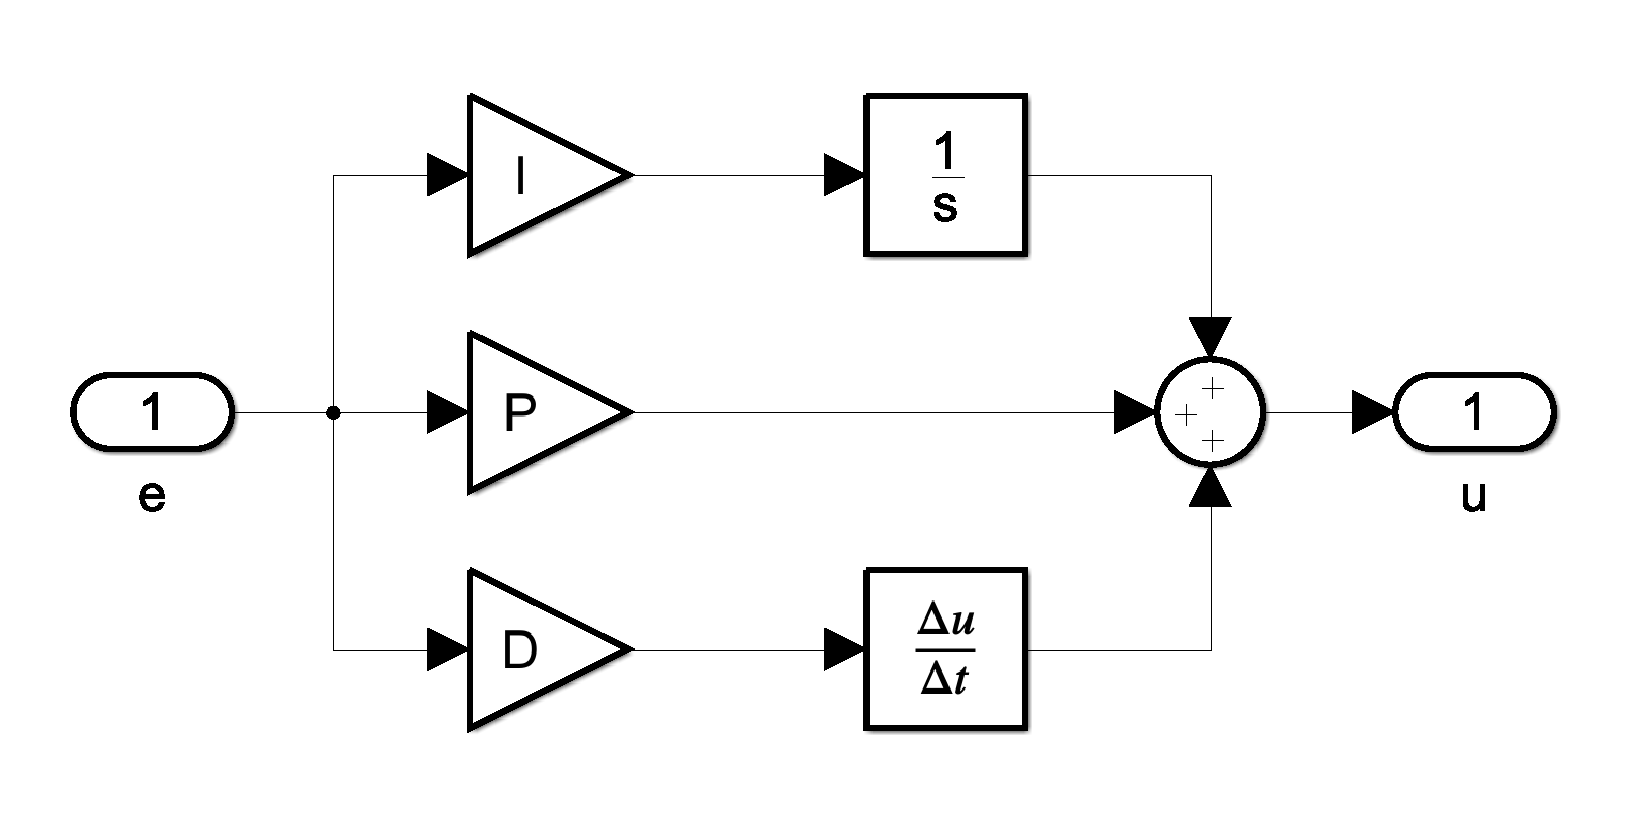
\includegraphics[scale=0.4]{PID_schema}
\caption{Bloková schéma PID regulátora}
\end{figure}

\pagebreak

\subsection{Filtrovaná derivácia}
Teoretická respektíve ideálna derivácia reprezentovaná operátorom $s$, tak ako vystupuje v rovnici \eqref{eq:PID}, nereprezentuje kauzálny systém a teda nie je ani numericky realizovateľná \footnote{Vysvetlenie prečo je to tak, sa ponecháva na čitateľa}.

Ideálnu deriváciu preto nahradíme filtrovanou deriváciou s prenosom:
\begin{equation}
\label{eq:filt_der}
	F_{der}(s)=\frac{Ns}{s+N}
\end{equation}

Pre parameter $N$ blížiaci sa k nekonečnu, bude filtrovaná derivácia blízka ideálnej:
\begin{equation}
	\lim_{N\to\infty}\frac{Ns}{s+N}=s
\end{equation} 

Po aplikácii filtrovanej derivácie \eqref{eq:filt_der} získame prenosovú funkciu regulátora:
\begin{equation}
 \label{eq:PID_filt}
 F_{reg}(s)=\frac{u(s)}{e(s)}=P+ I\frac{1}{s}+D \frac{Ns}{s+N}
\end{equation}


Ekvivalentná bloková schéma regulátora potom bude vyzerať nasledovne:
\begin{figure}[ht]
\centering
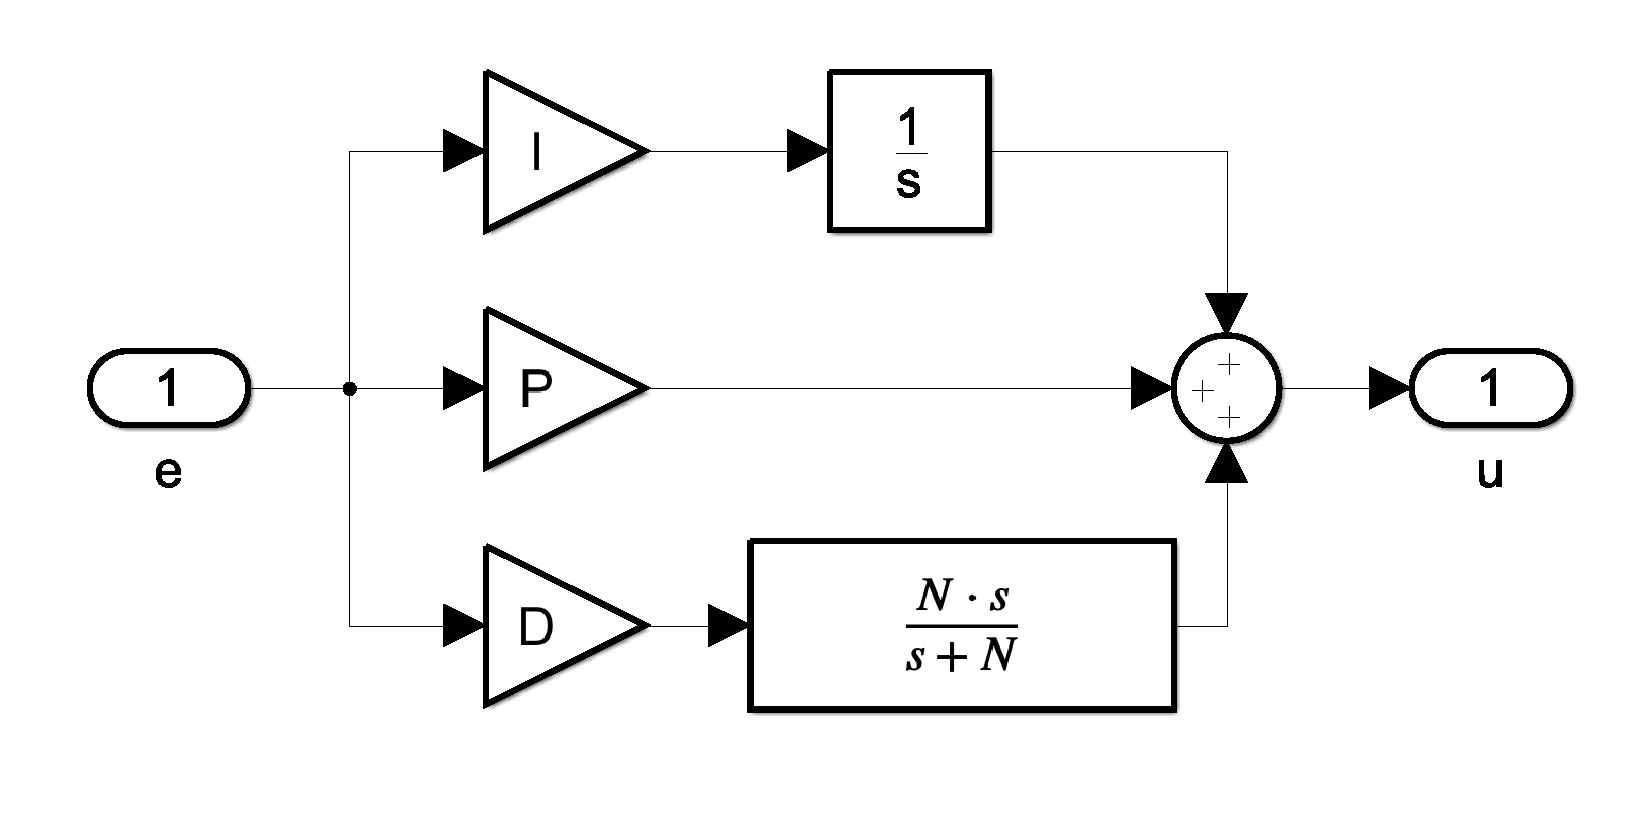
\includegraphics[scale=0.4]{PID_schema_filt}
\caption{Bloková schéma PID regulátora s realizovateľnou deriváciou}
\end{figure}

V ďalšom texte však budeme pre zjednodušenie uvažovať pôvodnú formu regulátora \eqref{eq:PID} s ideálnou deriváciou, respektíve parameter $N$ bude ``dostatočne veľký''.

\section{Prenosová funkcia prvého rádu}
Riadený systém nech je lineárny systém prvého rádu v tvare prenosovej funkcie:
\begin{equation}
\label{eq:system_TF}
  F_s=\frac{y(s)}{u(s)}=\frac{K}{Ts+1}
\end{equation}
Kde $K$ je zosilnenie a $T$ je časová konštanta systému.
Prechodová charakteristika takéhoto systému je aperiodická nakoľko systém obsahuje jeden reálny pól.

\pagebreak

\section{Uzavretý regulačný obvod}
Otvorený regulačný obvod (ozačovaný aj skratkou ORO) reprezentuje prenos systému bez zapojenia spätnej väzby.
Všeobecne je definovaný ako súčin prenosu regulátora a riadeného systému.

\begin{equation}
\label{eq:ORO}
F_{oro}(s)=F_{reg}(s)\:F_{s}(s)
\end{equation}

Uzavretý regulačný obvod (ozačovaný aj skratkou URO) je tvorený PID regulátorm, riadeným systémom a rozdielovým členom pre výpočet regulačnej odchýlky \eqref{eq:e}. Regulačný obvod sa nazýva uzavretý, nakoľko sa využíva spätná väzba z výstupu systému $y(t)$. 

Ekvivalentná bloková schéma URO bude vyzerať nasledovne:

\begin{figure}[ht]
\centering
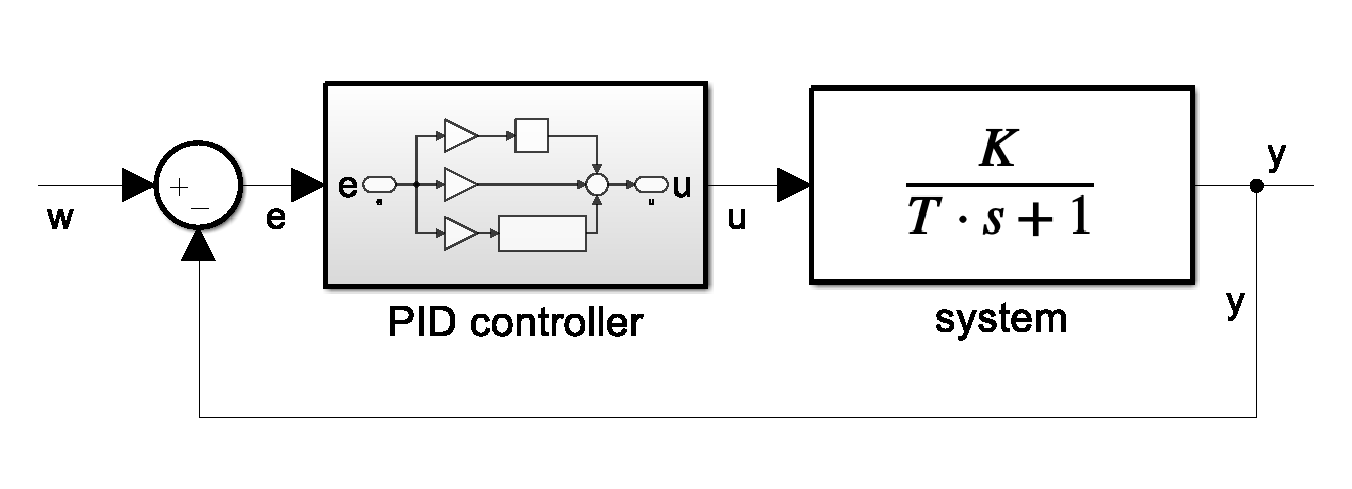
\includegraphics[scale=0.5]{PID_URO}
\caption{Bloková schéma uzavretého regulačného obvodu}
\end{figure}

Signály v typickom URO označujeme nasledovne:
\begin{itemize}
\item riadená velična $y(t)$
\item žiadaná hodnota  $w(t)$
\item regulačná odchýlka $e(t)$ - rovnica \eqref{eq:e}
\item akčný zásah $u(t)$
\end{itemize}

Prenosovú funkciu URO je všeobecne možné určiť ako:
\begin{equation}
 \label{eq:URO}
 F_{uro}(s)=\frac{y(s)}{w(s)}=\frac{F_{oro}}{1+F_{oro}\:F_{sv}}
\end{equation}

Kde $F_{sv}$ reprezentuje prenos samotnej spätnej väzby (v tomto prípade je rovný 1).
Aby sme mohli považovať riadenie za ''správne fungujúce`` musí spĺňať podmienku stability a podmienku nulovej trvalej regulačnej odchýlky $e(\infty)=0$. 

Stabilitu URO je možné posúdiť na základe analýzy pólov resp. koreňov menovateľa prenosu \eqref{eq:URO}:
\begin{equation}
 \label{eq:URO_stability}
 	 1+F_{oro}\:F_{sv}=0
\end{equation}
Pre stabilné riadenie musí mať každý z týchto koreňov zápornú reálnu časť.
Trvalú regulačnú odchýlku vieme posúdiť na základe statického zosilnenia prenosu URO. Toto zosilnenie by v prípade nulovej trvalej regulačnej odchýlky malo byť jednotkové.

Ďalej si ukážeme možnosti riadenia systému prvého rádu v tvare prenosovej funkcie \eqref{eq:system_TF} rôznymi variantami PID regulátora.

Nech sú parametre riadeného systému \eqref{eq:system_TF} zvolené ako $K=2$ a $T=5$ pre nasledujúce simulačné experimenty.

\pagebreak

\subsection{Riadenie prenosovej funkcie prvého rádu P regulátorom}

Aplikovaním rovnice pre PID regulátor \eqref{eq:PID} a uvažovaním parametrov $I=0$ a $D=0$, rovnice riadeného systému \eqref{eq:system_TF} a rovnice \eqref{eq:URO} získavame prenosovú funkciu URO.

\begin{equation}
\label{eq:URO_P}
 F_{uro}(s)=\frac{KP}{Ts+1+KP}
\end{equation}

Prenosová funkcia URO \eqref{eq:URO_P} reprezentuje systém prvého rádu, preto bude riadenie mať aperiodický charakter. Z hľadiska kvality regulácie je v tomto prípade prítomná trvalá regulačná odchýlka nakoľko statické zosilnenie $\frac{KP}{1+KP}$ je vždy menšie ako jedna.
Zvyšovaním zosilnenia proporcionálnej zložky $P$ trvalú regulačnú odchýlku zmenšujeme  avšak ju úplne neodstránime.
Čo sa týka stability riadenia, je možné ju posúdiť na základe analýzy koreňov menovateľa prenosovej funkcie URO \eqref{eq:URO_P}.  
\begin{equation}
\begin{array}{l}
 	Ts+1+KP=0 \\
 	s=-\frac{1+KP}{T}\\
\end{array}	
\end{equation}
Pre stabilné riadenie musí platiť:
\begin{equation}
-\frac{1+KP}{T}<0\\
\end{equation}

Zvolíme parameter regulátora ako $P=2$ a odsimulujeme priebeh riadenia.

\begin{figure}[ht]
\centering
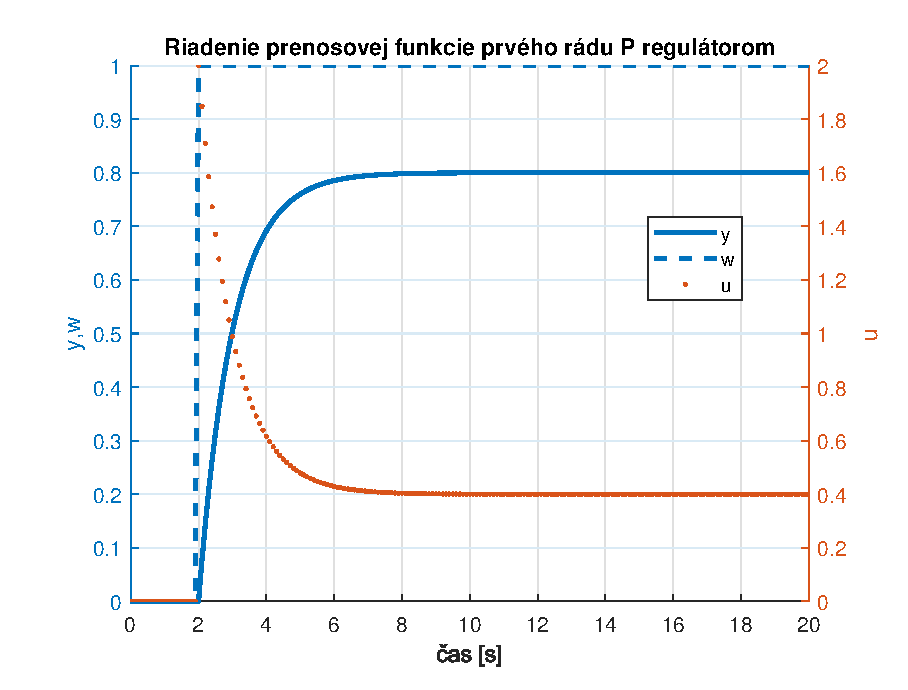
\includegraphics[scale=0.55]{P_control}
\end{figure}

Analyzujeme rozloženie pólov a núl prenosu URO:
\begin{figure}[ht]
\centering
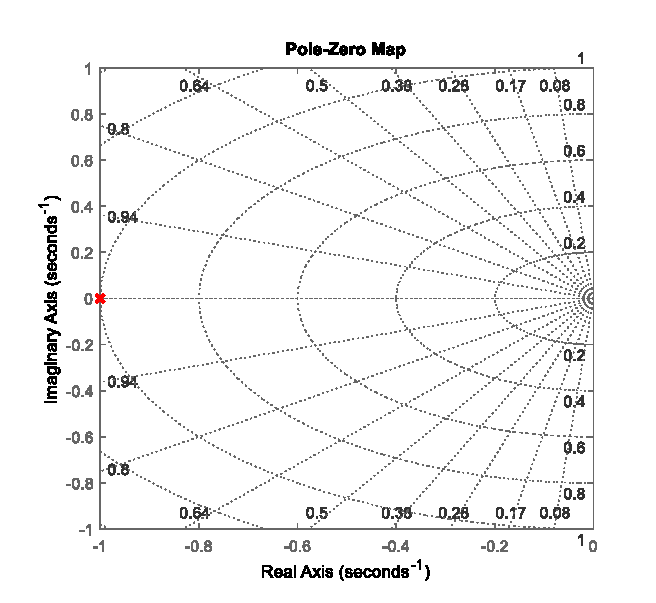
\includegraphics[scale=0.75]{pzmap_P}
\end{figure}

Odsimulovaný priebeh riadenia preukazuje predpokladanú trvalú regulačnú odchýlku a aperiodický charakter.
Z tohto dôvodu je P regulátor nevhodný pre riadenie takéhoto typu systému.

\pagebreak

\subsection{Riadenie prenosovej funkcie prvého rádu I regulátorom}

Aplikovaním rovnice pre PID regulátor \eqref{eq:PID} a uvažovaním parametrov $P=0$ a $D=0$, rovnice riadeného systému \eqref{eq:system_TF} a rovnice \eqref{eq:URO} získavame prenosovú funkciu URO.

\begin{equation}
\label{eq:URO_I}
F_{uro}(s)=\frac{KI}{Ts^2+s+KI}
\end{equation}

Prenosová funkcia \eqref{eq:URO_I} zväčša reprezentuje periodický systém druhého rádu. Z hľadiska kvality regulácie v tomto prípade nie je prítomná trvalá regulačná odchýlka nakoľko statické zosilnenie je rovné jednej.
Zvyšovaním zosilnenia integračnej zložky $I$ sa však zvyšuje kmitavosť riadenia.

Čo sa týka stability riadenia, tú je možné posúdiť na základe analýzy koreňov menovateľa prenosovej funkcie URO \eqref{eq:URO_I}. 

\begin{equation}
  Ts^2+s+KI=0
\end{equation} 

Póly určíme ako korene kvadratickej rovnice:
\begin{equation}
  s_{1,2}=\frac{-1\pm \sqrt{1-4TKI}}{2T}
\end{equation}

Zvolíme parameter regulátora ako $I=5$ a odsimulujeme priebeh riadenia.
\begin{figure}[ht]
\centering
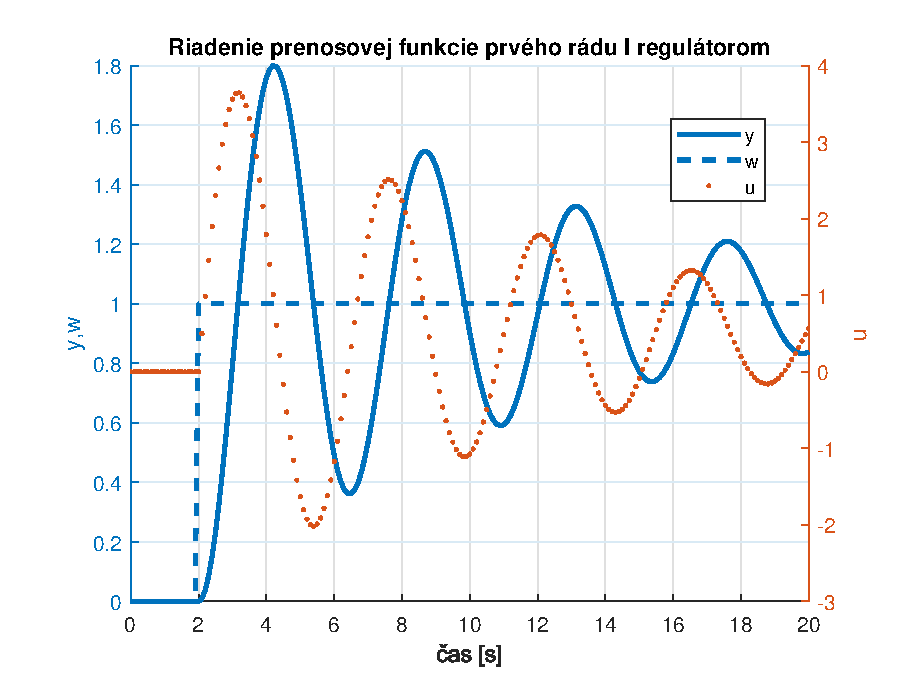
\includegraphics[scale=0.55]{I_control}
\end{figure}

Analyzujeme rozloženie pólov a núl prenosu URO:
\begin{figure}[ht]
\centering
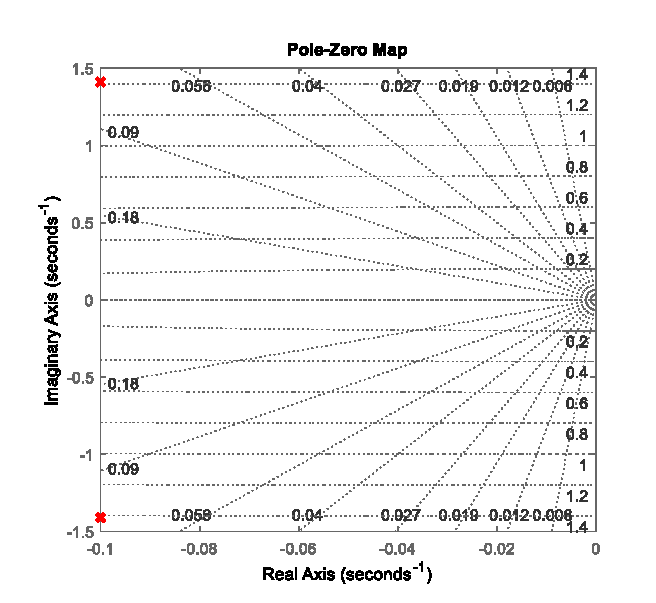
\includegraphics[scale=0.75]{pzmap_I}
\end{figure}

Hoci odsimulovaný priebeh riadenia preukazuje nulovú trvalú regulačnú odchýlku má však výrazne kmitavý charakter.
Z tohto dôvodu je I regulátor nevhodný pre riadenie takéhoto typu systému.

\pagebreak

\subsection{Riadenie prenosovej funkcie prvého rádu PI regulátorom}

Aplikovaním rovnice pre PID regulátor \eqref{eq:PID} s uvažovaním parametra $D=0$, rovnice riadeného systému \eqref{eq:system_TF} a rovnice \eqref{eq:URO} získaveme prenosovú funkciu URO.

\begin{equation}
\label{eq:URO_PI}
F_{uro}(s)=\frac{KPs+KI}{Ts^2+\left(KP+1\right)s+KI}
\end{equation}

Prenosová funkcia \eqref{eq:URO_PI} reprezentuje systém druhého rádu, preto riadenie môže mať periodický charakter ale aj aperiodický charakter (podľa konkrétneho rozloženia pólov). Z hľadiska kvality regulácie vďaka integračnej zložke nie je prítomná trvalá regulačná odchýlka nakoľko statické zosilnenie je rovné jednej.
Proporcionálna zložka riadenia je zodpovedná za rýchlosť vyregulovania ale aj za tlmenie kmitov. Zvyšovaním zosilnenia integračnej zložky sa naopak zvyšuje kmitavosť riadenia.
V prenosovej funkcii je prítomná aj ``nula'' systému teda koreň čitateľa.

Čo sa týka stability riadenia, tú je možné posúdiť na základe analýzy koreňov menovateľa prenosovej funkcie URO \eqref{eq:URO_PI}.  

\begin{equation}
  Ts^2+\left(KP+1\right)s+KI=0
\end{equation} 

Korene určíme ako korene kvadratickej rovnice:
\begin{equation}
  s_{1,2}=\frac{-\left(KP+1\right)\pm \sqrt{\left(KP+1\right)^2-4TKI}}{2T}
\end{equation}

Zvolíme parametre regulátora ako $P=2$ a $I=1.5$ a odsimulujeme priebeh riadenia.

\begin{figure}[ht]
\centering
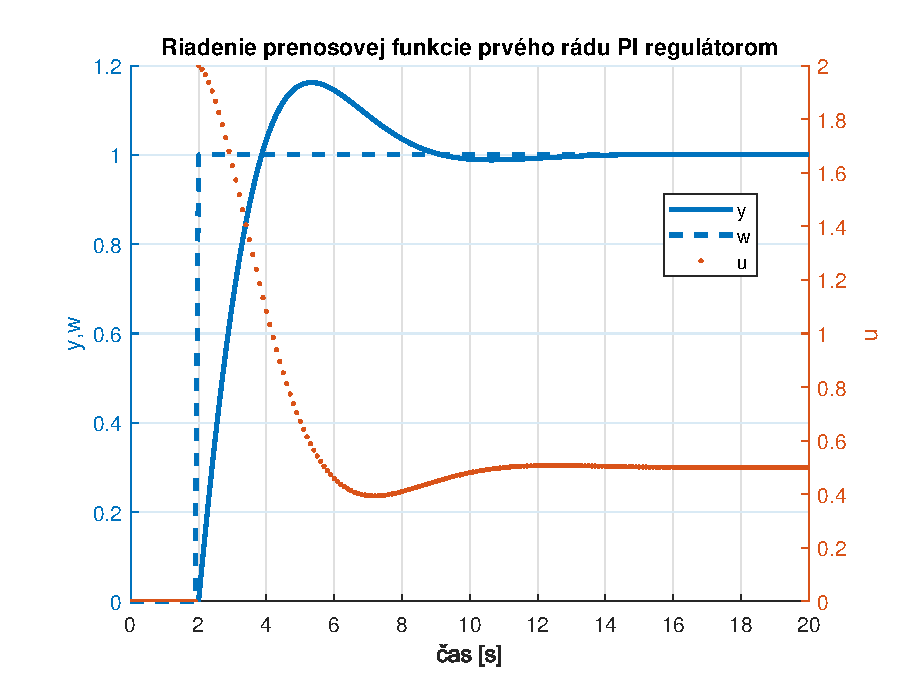
\includegraphics[scale=0.55]{PI_control}
\end{figure}

Analyzujeme rozloženie pólov a núl prenosu URO:

\begin{figure}[ht]
\centering
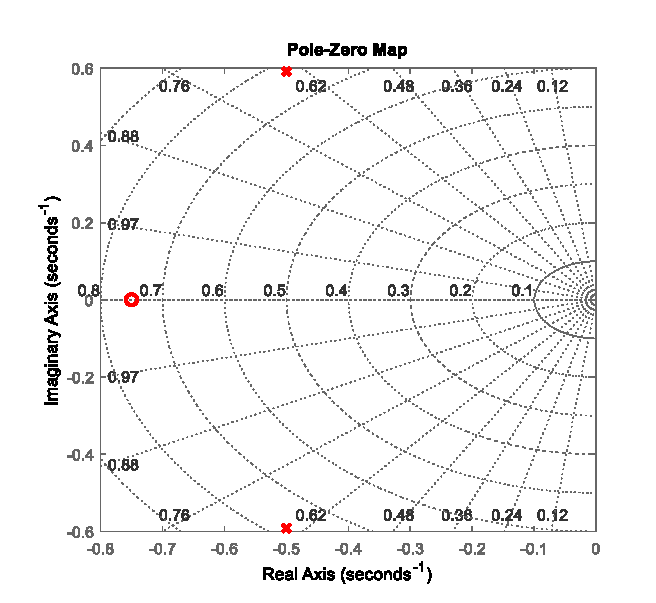
\includegraphics[scale=0.75]{pzmap_PI}
\end{figure}

Odsimulovaný priebeh riadenia preukazuje nulovú trvalú regulačnú odchýlku a má výrazne tlmený periodický charakter. Rovnako je tu prítomné aj mierne preregulovanie.
V globále je však PI regulátor vhodný pre riadenie systému prvého rádu.

\pagebreak

\subsection{Riadenie prenosovej funkcie prvého rádu PID regulátorom}

Aplikovaním rovnice pre PID regulátor \eqref{eq:PID}, rovnice riadeného systému \eqref{eq:system_TF} a rovnice \eqref{eq:URO} získavame prenosovú funkciu URO.

\begin{equation}
\label{eq:URO_PID}
F_{uro}(s)=\frac{KDs^2+KPs+KI}{\left(T+KD\right)s^2+\left(PK+1\right)s + KI}
\end{equation}

Prenosová funkcia \eqref{eq:URO_PID} reprezentuje systém druhého rádu, preto riadenie môže mať periodický charakter ale aj aperiodický charakter (podľa konkrétneho rozloženia pólov). Z hľadiska kvality regulácie vďaka integračnej zložke nie je prítomná trvalá regulačná odchýlka nakoľko statické zosilnenie je rovné jednej.
V prenosovej funkcii sú kvôli derivačnej zložke prítomné aj dve ``nuly'' systému a teda korene čitateľa zapríčiňujúce ``derivačný'' charakter prenosu riadenia.

Derivačná zložka však nevhodným spôsobom zvyšuje citlivosť riadenia na šum a zvyšuje nároky na dynamiku akčného zásahu.

Čo sa týka stability riadenia, tú je možné posúdiť na základe analýzy koreňov menovateľa prenosovej funkcie URO \eqref{eq:URO_PID}.

\begin{equation}
 \left(T+KD\right)s^2+\left(PK+1\right)s + KI=0
\end{equation}

Zvolíme parametre regulátora ako $P=2$ , $I=1$ , $D=1.5$ a odsimulujeme priebeh riadenia.

\begin{figure}[ht]
\centering
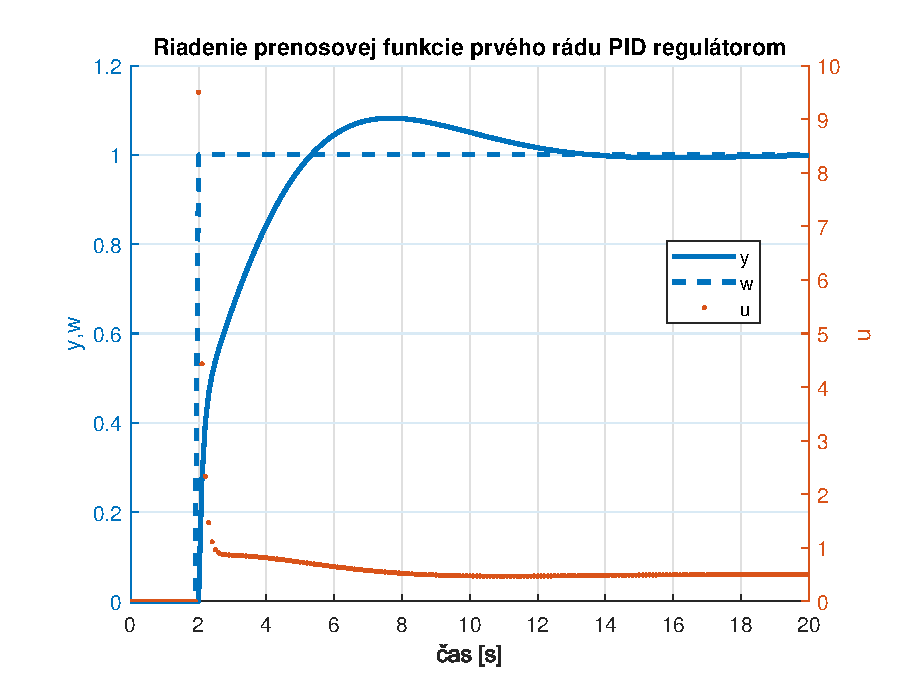
\includegraphics[scale=0.55]{PID_control}
\end{figure}

Analyzujeme rozloženie pólov a núl prenosu URO:
\begin{figure}[ht]
\centering
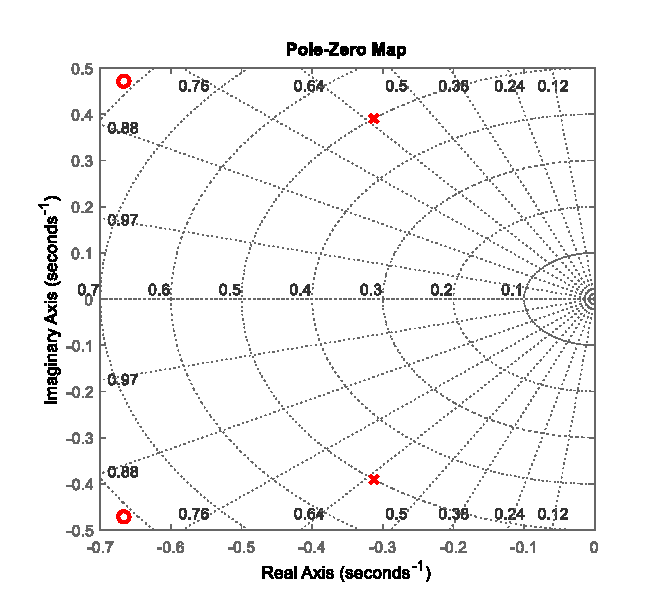
\includegraphics[scale=0.75]{pzmap_PID}
\end{figure}


Odsimulovaný priebeh riadenia preukazuje nulovú trvalú regulačnú odchýlku a má výrazne tlmený periodický charakter.
Akčný zásah však má na začiatku riadenia charakter impulzu. Tento jav je spôsobený prítomnosťou derivačnej zložky regulátora.
V princípe teda derivačná zložka regulátora nie je pre pre riadenie takéhoto typu systému potrebná.

\end{document}